\chapter{Theoretical Background}
\section{Definitions}
\subsection{Diffraction}
ADD IMAGES

A wave is the spatial propagating variation or rather perturbation or also an oscillation of a location-and time-dependent physical quantity. In Mathematics, when talking about a wave, we are referring to the so called wavefunction  $y(x,t) = A sin(wt - kx)$ which is a solution for the so called wave-equation. In general, this function depends on the location $x$ and in time $t$. The maximal amplitude / magnitude of a wave is denoted by $A$. The phase of wave indicates in which part within its period with respect to a reference point in time / location the wave is located.
Naturally occurring waves are uncommonly purely monochromatic waves, rather an overlapping of many waves with different wavelengths, which is denoted by interference. Interference  is a phenomenon in which two waves superimpose to form a resultant wave of greater or lower amplitude. All portions of these corresponding wavelengths are forming the so called spectrum. For example sunlight which is a overlapping of many electromagnetic monochromatic waves of different wavelengths, ranging continuously from infrared across visible light to ultraviolet. Thereby, many effects may occur like interference - by overlapping two waves they either will amplify or cancel out partially or even totally each other in some location.
Waves can experience in a different way a change in their form of appearance through reflexion, transmission, refraction or diffraction. In this thesis we are interested in particular in the bending of waves the so called effect of diffraction, which cannot be modeled using the standard ray theory of light.

When a wavefront is occluded partially by an obstacle, the wave is not only moving in the direction provided by the ray geometry, but also occur complex wave-movements outside of the geometric ray boundaries. This occurrence is called diffraction and occurs on the border of the wave's obstacle. 

Generally, the effect of diffraction occurs on the border of obstacle whenever a propagating wave encounters that obstacle. But its effects are generally most pronounced for waves whose wavelength is roughly similar to the dimensions of the diffracting objects. Conversely, if wavelength is hardly similar, then there is almost no diffraction at all. 
This implies diffraction occurs mostly when the surface detail is highly anisotropic. If the obstructing object provides multiple, closely spaced openings, a complex pattern of varying intensity can result. This is due to the superposition, or interference, of different parts of a wave that travels to the observer by different paths.

Example:
Light rays passing through a small aperture will begin to diverge and interfere with one another. This becomes more significant as the size of the aperture decreases relative to the wavelength of light passing through, but occurs to some extent for any aperture or concentrated light source.


\begin{figure}[H]
  \centering
  \subfigure[Large Aperture]{
  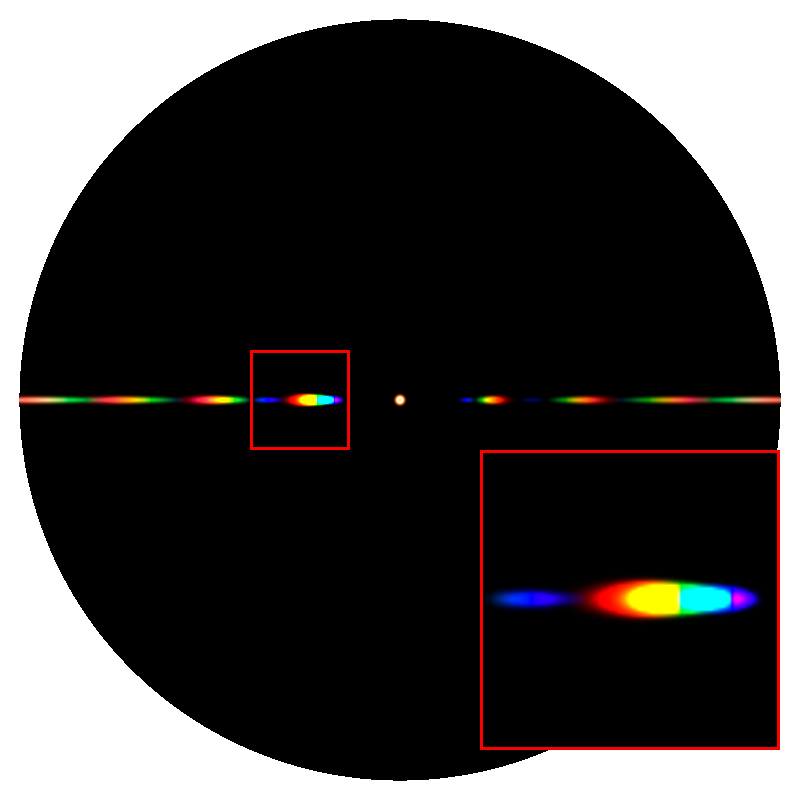
\includegraphics[scale=0.5]{1.png}
    \label{fig:diffractionLargeAperture}
  }
~
  \subfigure[Small Aperture]{
    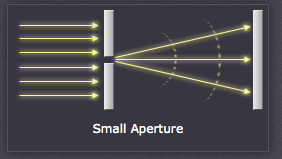
\includegraphics[scale=0.5]{2.png}
    \label{fig:diffractionSmallAperture}
  }
  \label{diffractionSingleSlitExample}
  \caption{Diffraction: Single Slit Example}
\end{figure}


Since the divergent rays now travel different distances, some move out of phase and begin to interfere with each other — adding in some places and partially or completely canceling out in others. This interference produces a diffraction pattern with peak intensities where the amplitude of the light waves add, and less light where they subtract. If one were to measure the intensity of light reaching each position on a line, the measurements would appear as bands similar to those shown below.

\begin{figure}[H]
  \centering
  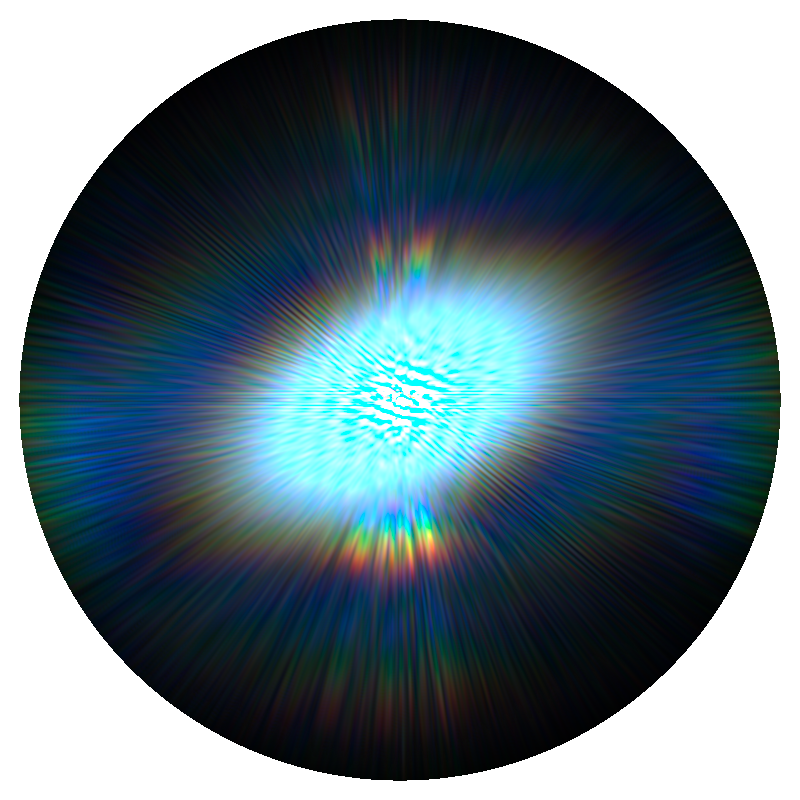
\includegraphics[scale=0.5]{3.png}
  \label{diffractionSingleSlitPattern}
  \caption{Diffraction Pattern}
\end{figure}

In general interference produces colorful effects due to the phase differences caused by a wave traversing thin media of different indices of refraction.

The effects of diffraction are often seen in everyday life. The most striking examples of diffraction are those that involve light; for example, the closely spaced tracks on a CD or DVD act as a diffraction grating to form the familiar rainbow pattern seen when looking at a disk

In optics, a diffraction grating is an optical component with a periodic structure, which splits and diffracts light into several beams travelling in different directions. The directions of these beams depend on the spacing of the grating and the wavelength of the light so that the grating acts as the dispersive element.
The relationship between the grating spacing and the angles of the incident and diffracted beams of light is known as the grating equation. See chapter Evaluation Data Acquisition for further insight.

\subsection{Radiometry}
Light is fundamentally a propagation form of energy, so it is useful to define the SI unit of energy which is joule (J). To aid our intuition, let us describe radiometry in terms of collections of large numbers of photons. A photon can be considered as a quantum of light that has a position, direction of propagation and a wavelength $\lambda$ measured in nanometers. A photon travels in a certain speed, denoted by $v = \frac{c}{n}$, that depends only on the refractive index $n$ of the medium through which it propagates and the speed of light $c$. This allows us do define the frequency $f = \frac{c}{\lambda}$. The amount of energy $q$ carried by a photon is given by the following relationship: $q = hf= \frac{hc}{\lambda}$ where $h$ is the Plank's constant.

\myparagraph{Spectral Energy}
If there is a large collection of photons given, their total energy $Q = \sum_i q_i$ is the sum of energies of each photon $q_i$ within the collection. But how is the energy distributed across wavelengths? One way in order to determine this distribution is to order all photons by their associated wavelength and then make a histogram from them. This is achieved by a discretization of their spectrum and combine all photons which will fall into the same interval, i.e. compute the sum for each interval from the energy of all their photons. By dividing such an interval by its length, denoted by $Q_\lambda$, we get a relatively scaled interval energy, which is called spectral energy and it is an intensive quantity. Intensive quantities can be thought of as density functions that tell the density of an extensive quantity at an infinitesimal point.

\myparagraph{Power}
Power is the estimated rate of energy production for light sources and is measured in the unit Watts, denoted by Q, which is another name for joules per second. Since power is a density over time, it is well defined even when energy production is varying over time. As with energy, we are really interested in the spectral power, measured in W/nm, denoted by $\Phi_\lambda$

\myparagraph{Irradiance}
The term irradiance comes into place when we are interested in \textit{how much light hits a given point}. In order to answer this question, we must make use of a density function. Let $\Delta A$ a finite area sensor that is smaller than the light field being measured. The spectral irradiance $E$ is just the power per unit area $\frac{\Delta \Phi}{\Delta A}$ which is 

\begin{equation}
 E = \frac{\Delta q}{\Delta A \Delta t \Delta \lambda}
\end{equation}

Thus the units of irradiance are $Jm^{-2}s^{-1}(nm)^{-1}$, the power per unit surface area.

\myparagraph{Radiance}

TODO: SHOW IMAGE: SOLID angle
$WIKI: http://en.wikipedia.org/wiki/Radiance$
$CG Slides 2012 - 6.shading$
$Book: Fundamentals of computer graphics$

Although irradiance tells us how much light is arriving at a point, it tells us little about the direction that light comes from. To measure something similar to what we see with our eyes we need to be able to associate the quantity \textit{how much light with a specific direction}. 

Radiance is a measure of the quantity of radiation that passes through or is emitted from a surface and falls within a given solid angle in a specified direction. Think of it as the energy carried along a narrow beam of light. 
This means radiance characterizes the total emission of reflectance. It indicates how much of the power emitted by a reflecting surface will be received by an optical system looking at the surface from some given angle of view. Formally, this leads us to the following definition of radiance: 

\begin{equation}
 L(\omega) = \frac{d^2 \Phi}{dA d\Omega cos(\theta)} \approx \frac{\Phi}{\Omega A cos(\theta)}
\end{equation}

where $L$ is the observed radiance in the unit energy per area per solid angle, which is $Wm^-2 sr^-1$ in direction $\omega$ which has an angle $\theta$ between the surface normal and $\omega$, $\Theta$ is the total flux or power emitted, $\theta$ is the angle between the surface normal and the specified direction, $A$ is the area of the surface and $\Omega$ is the solid angle in the unit steradian subtended by the observation or measurement.

It is useful to distinguish between radiance incident at a point on a surface and excitant from that point. Terms for these concepts sometimes used in the graphics literature are surface radiance $L_r$ for the radiance \textit{reflected} from a surface and field radiance $L_i$ for the radiance \textit{incident} at a surface.  

\myparagraph{BRDF}
\label{brdf}

The bidirectional reflectance distribution function, in short BRDF, denoted as $f_r(\omega_i, \omega_r)$ is a four dimensional function that defines \textit{how light is reflected at an opaque surface}. The function takes a negative directed incoming light direction, $\omega_{\text{i}}$, and outgoing direction, $\omega_{\text{r}}$ as input argument. Both are defined with respect to the surface normal $\mathbf{n}$.Hence A BRDF returns the ratio of reflected radiance exiting along $\omega_{\text{r}}$ to the irradiance incident on the surface from direction $\omega_{\text{i}}$, which is formally:
  
\begin{align}
  BRDF(\omega_i, \omega_r)
  & = f_r(\omega_i, \omega_r) \\
  & = \frac{dL_r(\omega_r)}{dE_i(\omega_i)} \\
  & = \frac{dL_r(\omega_r)}{L_i(\omega_i)cos(\theta_i)d\omega_i}
\end{align}

L is the reflected radiance, E is the irradiance and $\theta_{\text{i}}$ is the angle between $\omega_{\text{i}}$ and the surface normal, $\mathbf n$. The index $\text{i}$ indicates incident light, whereas the index $\text{r}$ indicates reflected light.

\myparagraph{Spectral Rendering}
In Computer Graphics, spectral rendering is where a scene's light transport is modeled considering the whole span of wavelengths instead of R,G,B values (still relating on geometric optic, which ignore wave phase). The motivation is that real colors of the physical world are spectrum; trichromatic colors are only inherent to Human Visual System.

In Computer Graphics, when talking about Spectral Rendering, we are referring to use the whole span of wavelengths instead just using RGB values in order for rendering a scene's light transport. The motivation for using the whole wavelength spectrum is due to the fact that trichromatic colors are only inherent to human visual system and therefore many phenomenons are poorly represented just using trichromy. 

\myparagraph{Colors}
\label{subsec:colors}
In order to see how crucial the role human vision plays, we only have to look the the definition of color: 
\textit{Color is the aspect of visual perception by which an observer may distinguish differences between two structure-free fields of view of the same size and shape such as may be caused by differences in the spectral composition of the radiant energy concerned in the observation}. -  Wyszechki and Siles, 2000 mentioned in Computer Graphics Fundamentals Book. 

An eye consists of photoreceptor cells, cones and rods. Cones are responsible for color perception. 
The human eye has three kinds of cone cells, with spectral sensitivity peaks in short (S, 420–440 nm), middle (M, 530–540 nm), and long (L, 560–580 nm) wavelengths.
In principle, any color sensation in human color perception can therefore be described by just three parameters, corresponding to levels of stimulus of the three types of cone cells.

A color space maps a range of physically produced colors from mixed light to an objective description of color
sensations registered in the eye in terms of tristimulus values.

Tristimulus values associated with a color space can be conceptualized as amounts of three primary colors in a tri-chromatic additive color model. In some color spaces (including LMS and XYZ spaces), the primary colors used are not real colors, in the sense that they cannot be generated with any light spectrum.

Due to distribution of cones in human eye, the tristimulus values depend on over's field of view. CIE defined a color mapping function called standard observer, to eliminate this variable represent an average human chromatic response.

\begin{figure}[H]
  \centering
  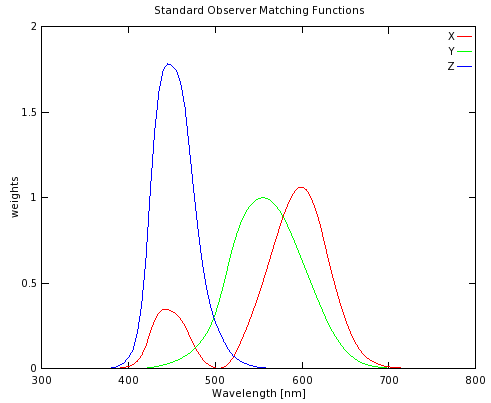
\includegraphics[scale=0.7]{background/somatchingfunctions.png}
  \label{fig:matchingfunction}
  \caption{Plots of our color matching functions we used for rendering}
\end{figure}

The CIE's color matching functions $\overline{x}(\lambda)$, $\overline{y}(\lambda)$, $\overline{z}(\lambda)$ are the numerical description of the chromatic response of the observer (described above). They can be thought of as the spectral sensitivity curves of three linear light detectors yielding the CIE tristimulus values X, Y and Z.

The tristimulus values for a color with a spectral power distribution $I(\lambda)$, are given in terms of the standard observer by:

\begin{align*}
    X= \int_{380}^{780} I(\lambda)\,\overline{x}(\lambda)\,d\lambda \\
    Y= \int_{380}^{780} I(\lambda)\,\overline{y}(\lambda)\,d\lambda \\
    Z= \int_{380}^{780} I(\lambda)\,\overline{z}(\lambda)\,d\lambda
\end{align*}

where $\lambda$, is the wavelength of the equivalent monochromatic light (measured in nanometers).

It is not possible to build a display that corresponds to CIE XYZ, for this reasons it is necessary to design  other color spaces, which are physical realizable, offers efficient encoding, are perceptual uniform and have an intuitive color specification. 

There are simple conversions between XYZ color space to any other color space defined, described as linear transformations.

\subsection{Signal Processing Basics}
A signal is a function that conveys information about the behavior or attributes of some phenomenon.
In the physical world, any quantity exhibiting variation in time or variation in space (such as an image) is potentially a signal that might provide information on the status of a physical system, or convey a message between observers.

The Fourier Transform is an important image processing tool which is used to decompose an image into its sine and cosine components. The output of the transformation represents the image in the Fourier or frequency domain, while the input image is the spatial domain equivalent. In the Fourier domain image, each point represents a particular frequency contained in the spatial domain image. 

\myparagraph{Fourier Transformation}
The Fourier-Transform is a mathematical tool which allows to transform a given function or rather a given signal from defined over a time- (or spatial-) domain into its corresponding frequency-domain.
 
Let $f$ an measurable function over $\mathds{R}^n$. Then, the continuous Fourier Transformation(\textbf{FT}), denoted as $\mathcal{F}\{f\}$ of $f$, ignoring all constant factors in the formula, is defined as:
 
\begin{equation}
  \mathcal{F}_{FT}\{f\}(w) = \int_{\mathds{R}^n} f(x)e^{-iwt} dt
\end{equation}

whereas its inverse transform is defined like the following which allows us to obtain back the original signal:

\begin{equation}
  \mathcal{F}_{FT}^{-1}\{f\}(w) = \int_{\mathds{R}} \mathcal{F}\{w\}e^{iwt} dt
\end{equation}

Usual $w$ is identified by the angular frequency which is  equal $w = \frac{2 \pi}{T} = 2 \pi v_f$. In this connection, $T$ is the period of the resulting spectrum and $v_f$ is its corresponding frequency.

By using Fourier Analysis, which is the approach to approximate any function by sums of simpler trigonometric functions, we gain the so called Discrete Time Fourier Transform (in short \textbf{DTFT}). The DTFT operates on a discrete function. Usually, such an input function is often created by digitally sampling a continuous function. The DTFT itself is operation on a discretized signal on a continuous, periodic frequency domain and looks like the following:

\begin{equation}
  \mathcal{F}_{DTFT}\{f\}(w) = \sum_{-\infty}^{\infty} f(x) e^{-iwk}
\end{equation}

Note that the DTFT is not practically suitable for digital signal processing since there a signal can be measured only in a finite number of points. Thus, we can further discretize the frequency domain and will get then the Discrete Fourier Transformation (in short \textbf{DFT}) of the input signal:

\begin{equation}
  \mathcal{F}_{DFT}\{f\}(w) = \sum_{n=0}^{N-1} f(x) e^{-iw_{n}k}
\end{equation}

Where the angular frequency $w_n$ is defined like the following $w_n = \frac{2\pi n}{N}$ and $N$ is the number of samples within an equidistant period sampling.

Any continuous function $f(t)$ can be expressed as a series of sines and cosines. This representation is called the Fourier Series (denoted by $FS$) of $f(t)$.
\begin{equation}
  f(t) = \frac{1}{2}a_0 + \sum_{n=1}^{\infty} a_n cos(nt) + \sum_{n=1}^{\infty} b_n cos(nt)
\end{equation}

where

\begin{align*}
    a_0 = \int_{-\pi}^{\pi} f(t) dt \\
    a_n = \frac{1}{\pi}\int_{-\pi}^{\pi} f(t) cos(nt) dt \\
    b_n = \frac{1}{\pi}\int_{-\pi}^{\pi} f(t) sin(nt) dt \\
\end{align*}

\myparagraph{Convolution}
The convolution $f*g$ of two functions $f$, $g$$\colon \mathds{R}^n \to \mathds{C} $ is defined as:  
\begin{equation}
  \mathcal (f*g)(t) = \int_{\mathds{R}^n} f(t)g(t-x) dx
\end{equation}

Note that the Fourier transform of the convolution of two functions is the product of their Fourier transforms. This is equivalent to the fact that Convolution in spatial domain is equivalent to multiplication in frequency domain. Therefore, the inverse Fourier transform of the product of two Fourier transforms is the convolution of the two inverse Fourier transforms

Last an illustration of the relationships between the previous presented Fourier transformations and different given input signals. First an concrete example shown in Figure $\ref{fig:contdiscft}$. Table $\ref{tab:ftoperatorsdependencies}$ tells what Fourier transformation operator has to be applied to which kind of input signal and what properties its resulting Fourier transform will have.

% image from wikipedia
\begin{figure}[H]
  \centering
  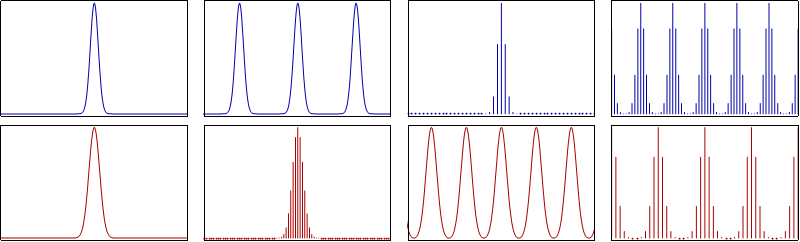
\includegraphics[scale=0.5]{background/dcft.png}
  \caption{Relationship between the continuous Fourier transform and the discrete Fourier transform: Left column: A continuous function (top) and its Fourier transform (bottom). Center-left column: Periodic summation of the original function (top). Fourier transform (bottom) is zero except at discrete points. The inverse transform is a sum of sinusoids called Fourier series. Center-right column: Original function is discretized (multiplied by a Dirac comb) (top). Its Fourier transform (bottom) is a periodic summation (DTFT) of the original transform. Right column: The DFT (bottom) computes discrete samples of the continuous DTFT. The inverse DFT (top) is a periodic summation of the orginal samples.}
\label{fig:contdiscft}
\end{figure}

\begin{table}[H]
    \begin{tabular}{l|l|l}
    \hline
    Spetail signal $f(t)$ is & Operator & Transformed frequency signal $\hat{f}(\omega)$ is\\
    \hline
    continuous and periodic in $t$ & FS & only discrete in $\omega$ \\
    only continuous in $t$ & FT & only continuous in $\omega$\\
    only discrete in $t$ & DTFT & continuous and periodic in $\omega$\\
    discrete and periodic in $t$ & DFT & discrete and periodic in $\omega$\\
    \hline
    \end{tabular}
\caption{Fourier operator to apply for a given spatial input signal and the properties of its resulting output signal in frequency space}
\label{tab:ftoperatorsdependencies}
\end{table}

\myparagraph{Taylor Series}
Taylor series is a representation of a function as an infinite sum of terms that are calculated from the values of the function's derivatives at a single point.

The Taylor series $\mathcal T$ of a real or complex-valued function ƒ(x) that is infinitely differentiable at a real or complex number $a$ is the power series:
\begin{equation}
  \mathcal T(f;a)(x) = \sum_{n=0}^{\infty} \frac{f^{n}(a)}{n!}(x-a)^n
\end{equation}


\section{Thesis Basis: J.Stam's Paper about Diffraction Shader}
In his paper about Diffraction Shader, J. Stam derives a BRDF which is modeling the effect of diffraction for various analytical anisotropic reflexion models relying on the so called scalar wave theory of diffraction for which a wave is assumed to be a complex valued scalar. 
It's noteworthy, that Stam's BRDF formulation does not take into account the polarization of the light. Fortunately, light sources like sunlight and light bulbs are unpolarized. 

A further assumption in Stam's Paper is, the emanated waves from the source are stationary, which implies the wave is a superposition of independent monochromatic waves. This implies that each wave is associated to a definite wavelength lambda. However, sunlight once again fulfills this fact.

In our simulations we will always assume we have given a directional light source, i.e. sunlight. Hence, Stam's model can be used for our derivations.

For his derivations Stam uses the Kirchhoff integral (ADD REF TO WIKI), which is relating the reflected field to the incoming field. This equation is a formalization of Huygen’s well-known principle that states that if one knows the wavefront at a given moment, the wave at a later time can be deduced by considering each point on the first wave as the source of a new disturbance. Mathematically speaking, once the field  $\psi_1 =  e^{ik\mathbf{x} \cdot \mathbf{s}\mathbf{s}}$ on the surface is known, the field $\psi_2$ everywhere else away from the surface can be computed.
More precisely, we want to compute the wave $\psi_2$ equal to the reflection of an incoming planar monochromatic wave $\psi_1 = e^{ik \omega_i * x}$  traveling in the direction $\omega_i$ from a surface $S$ to the light source. Formally, this can be written as:

\begin{equation}
\psi_{2}(\omega_i, \omega_r) = \frac{i k e^{i K R}}{4 \pi R} (F(-\omega_i-\omega_r)-(-\omega_i+\omega_r)) \cdot I_{1}(\omega_i, \omega_r) 
\label{eq:kirchhoff}
\end{equation}

with

\begin{equation}
I_{1}(\omega_i, \omega_r) = \int_{S} \hat{\mathbf{n}} e^{ik(-\omega_i-\omega_{r}) \cdot \mathbf{s} d\mathbf{s}}
\label{eq:IBase}
\end{equation}

In applied optics, when dealing with scattered waves, one does use differential scattering cross-section rather than defining a BRDF which has the following identity: 

\begin{equation}
    \sigma^0 = 4 \pi \lim_{R \to \infty} R^2 \frac{\langle \left|\psi_2\right|^2\rangle}{\langle \left|\psi_1\right|^2\rangle}
\end{equation}

where R is the distance from the center of the patch to the receiving point $x_p$, $\hat{\mathbf{n}}$ is the normal of the surface at s and the vectors:

The relationship between the BRDF and the scattering cross section can be shown to be equal to 

\begin{equation}
 BRDF = \frac{1}{4\pi}\frac{1}{A}\frac{\sigma^0}{cos(\theta_i)cos(\theta_r)}
 \label{fig:crossscateringbrdfrelationship} 
\end{equation}

where $\theta_i$ and $\theta_r$ are the angles of incident and reflected directions on the surface with the surface normal $n$. See ~\ref{fig:geometricsetup}.

\begin{figure}[ht]
  \centering
  
\includegraphics[scale=0.25]{brdfdiagram.png}
  \caption{$\omega_i$ points toward the light source, $\omega_r$ points toward the camera, $n$ is the surface normal}
  \label{fig:geometricsetup}  
\end{figure}

The components of vector resulting by the difference between these direction vectors:
In order to simplify the calculations involved in his vectorized integral equations, Stam considers the components of vector 
\begin{equation}
  (u,v,w) = -\omega_i - \omega_r 
\label{eq:uvw}
\end{equation}

explicitly and introduces the equation: 
\begin{equation}
  I(ku,kv) = \int_{S} \hat{\mathbf{n}} e^{ik(u,v,w) \cdot \mathbf{s} d\mathbf{s}} 
\label{eq:Istart}
\end{equation}

which is a first simplification of $\ref{eq:IBase}$. Note that the scalar $w$ is the third component of ~\ref{eq:uvw} and can be written as $w = -(cos(\theta_i)+cos(\theta_r))$ using spherical coordinates. The scalar $k=\frac{2\pi}{\lambda}$ represent the wavenumber.


During his derivations, Stam provides a analytical representation for the Kirchhoff integral assuming that each surface point $s(x,y)$ can be parameterized by $(x,y,h(x,y))$ where $h$ is the height at the position $(x,y)$ on the given $(x,y)$ surface plane. Using the tangent plane approximation for the parameterized surface and plugging it into $\ref{eq:Istart}$ he will end up with: 

\begin{equation}
    \mathbf{I}(ku, kv) = \int \int (-h_{x}(x,y), -h_{y}(x,y), 1) e^{ikwh(x,y)} e^{ik(ux + vy)} dx dy
\label{eq:I1}
\end{equation}

For further simplification Stam formulates auxillary function which depends on the provided height field: 
\begin{equation}
  p(x,y) = e^{iwkh(x,y)} 
\label{eq:px}
\end{equation}

which will allow him to further simplify his equation $\ref{eq:I1}$ to:

\begin{equation}
    \mathbf{I}(ku, kv) = \int \int \frac{1}{ikw}(-p_x, -p_y, ikwp) dx dy
\label{eq:I2}
\end{equation}

where he used that $(-h_{x}(x,y), -h_{y}(x,y), 1)e^{kwh(x,y)}$ is equal to $\frac{(-p_x, -p_y, ikwp)}{ikw}$ using the definition of the partial derivatives applied to the function $\ref{eq:px}$.

Let $P(x,y)$ denote the Fourier Transform (FT) of $p(x,y)$. Then, the differentiation with respect to x respectively to y in the Fourier domain is equivalent to a multiplication of the Fourier transform by $-iku$ or $-ikv$ respectively. This leads him to the following simplification for $\ref{eq:I1}$:

\begin{equation}
    \mathbf{I}(ku, kv) = \frac{1}{w}P(ku, kv) \cdot (u,v,w)
\label{eq:I3}
\end{equation}

Let us consider the term $g = (F(-\omega_i - \omega_r)-(-\omega_i + \omega_r))$, which is a scalar factor of $\ref{eq:kirchhoff}$. The dot product with $g$ and $(-\omega_i - \omega_r)$ is equal $2F(1 + \omega_i \cdot \omega_r)$. Putting this finding and the identity $\ref{eq:I3}$ into $\ref{eq:kirchhoff}$ he will end up with:

\begin{equation}
\psi_{2}(\omega_i, \omega_r) = \frac{i k e^{i K R}}{4 \pi R} \frac{2F(1 + \omega_i \cdot \omega_r)}{w} P(ku, kv)
\label{eq:kirchhoffFinding}
\end{equation}

By using the identity $\ref{fig:crossscateringbrdfrelationship}$, this will lead us to his main finding:
\begin{equation} 
  BRDF_{\lambda}(\omega_i, \omega_r) = \frac{k^2 F^2 G}{4\pi^2 A w^2} \langle \left|P(ku, kv)\right|^2\rangle
\label{eq:mainstam}
\end{equation}

where $G$ is the so called geometry term which is equal: 

\begin{equation}
  G =\frac{(1 + \omega_i \cdot \omega_r)^2}{cos(\theta_i)cos(\theta_r)}
\label{eq:geometricterm}
\end{equation}

\section{Derivations}
\subsection{BRDF formulation}
Lets assume we have given an incoming light source with solid angle $\omega_i$, $\theta{_i}$ is its angle of incidence, $\omega_r$ is the solid angle for the reflected light, $\lambda$ wavelength, $\Omega$ is the hemisphere we of integration for the incoming light. Then, we are able to formulate a BRDF by using its definition:  



\begin{alignat}{4}
& f_r(\omega_i, \omega_r) &&= \frac{dL_r(\omega_r)}{L_i(\omega_i)cos(\theta_i)d\omega_i} \nonumber \\
\Rightarrow{} & f_r(\omega_i, \omega_r) L_i(\omega_i)cos(\theta_i)d\omega_i &&= dL_r(\omega_r) \nonumber \\
\Rightarrow{} & \int_{\Omega}f_r(\omega_i, \omega_r) L_i(\omega_i)cos(\theta_i)d\omega_i &&= \int_{\Omega}dL_r(\omega_r) \nonumber\\
\Rightarrow{} & L_r(\omega_r) &&= \int_{\Omega}f_r(\omega_i, \omega_r) L_i(\omega_i)cos(\theta_i)d\omega_i
\end{alignat}

The last equation is the so called rendering equation.
We assume further, that our incident light is a directional, unpolarized light source like sunlight and therefore its radiance is given as 

\begin{equation}
 L_{\lambda}(\omega)=I(\lambda)\delta(\omega-\omega_i)
\end{equation}

where $I(\lambda)$ is the intensity of the relative spectral power for the wavelength $\lambda$. 
Since all light rays are parallel whenever we are provided by a directional light source and we can think of radiance as a measure of the light emitted from a particular surface location into a particular direction, above's radiance identity will follow immediately. 
By plugging this identity into our current rendering equation, we will get:

\begin{align}
L_{\lambda}(w_r) 
& = \int_{\Omega} BRDF_{\lambda}(\omega_i, \omega_r) L_{\lambda}(\omega_i) cos(\theta_i) d\omega_i \nonumber \\
& = BRDF_{\lambda}(\omega_i, \omega_r) I(\lambda) cos(\theta_i)
\end{align}

where $L_{\lambda}(\omega_i)$ is the incoming radiance and $L_{\lambda}(\omega_r)$ is the radiance reflected by given surface
Note that above's integral vanishes since $\delta(\omega-\omega_i)$ is only equal one if and only if $\omega = \omega_i$.

For the $BRDF(\omega_i, \omega_r)$ we are going to use Stam's main derivation $~\eqref{eq:mainstam}$ applying the fact that the wavenumber is equal $k=\frac{2\pi}{\lambda}$:

\begin{align}
BRDF(\omega_i, \omega_r) 
& = \frac{k^2 F^2 G}{4\pi^2 A w^2} \langle \left|P(ku, kv) \right|^2\rangle \nonumber\\
& = \frac{k^2 F^2 (1 + \omega_i \cdot \omega_r)^2}{cos(\theta_i)cos(\theta_r) 4\pi^2 A w^2} \langle \left|P(ku, kv)  \right|^2\rangle \nonumber\\
& = \frac{4 \pi^2 F^2 (1 + \omega_i \cdot \omega_r)^2}{cos(\theta_i)cos(\theta_r) 4\pi^2 A \lambda^2 w^2} \langle \left|P(ku, kv)  \right|^2\rangle \nonumber\\
& = \frac{F(w_i, w_r)^2 (1 + \omega_i \cdot \omega_r)^2}{cos(\theta_i)cos(\theta_r) A \lambda^2 w^2} \langle \left|P(ku, kv)  \right|^2\rangle
\end{align}

going back to the definition of $(u,v,w)= -\omega_i - \omega_r$ and using spherical coordinates, we get for $w$ the following identity $w = -\omega_i - \omega_r = -(\omega_i + \omega_r) = -(cos(\theta_i)+cos(\theta_r))$ and therefore $w^2$ is equal $(cos(\theta_i)+cos(\theta_r))^2$
This new fact will allow us to get even further:

\begin{align}
L_{\lambda}(\omega_r) 
& = \frac{F(\omega_i, \omega_r)^2 (1 + \omega_i \cdot \omega_r)^2}{A \lambda^2 cos(\theta_i)cos(\theta_r)  (cos(\theta_i)+cos(\theta_r))^2} \langle \left|P_{cont}(\frac{2\pi u}{\lambda}, \frac{2\pi v}{\lambda})  \right|^2\rangle cos(\theta_i) I(\lambda) \nonumber \\
& = I(\lambda) \frac{F(\omega_i, \omega_r)^2 (1 + \omega_i \cdot \omega_r)^2}{\lambda^2 A (cos(\theta_i)+cos(\theta_r))^2 cos(\theta_r)} \langle \left|P_{cont}(\frac{2\pi u}{\lambda}, \frac{2\pi v}{\lambda})  \right|^2\rangle \nonumber \\
& = I(\lambda) \frac{F(\omega_i, \omega_r)^2 (1 + \omega_i \cdot \omega_r)^2}{\lambda^2 A (cos(\theta_i)+cos(\theta_r))^2 cos(\theta_r)} \langle \left|T_0^2 P_{dtft}(\frac{2\pi u}{\lambda}, \frac{2\pi v}{\lambda})  \right|^2\rangle
\end{align}

$P_{cont}$ denotes the continuous inverse Fourier-Transform for the Taylor-Series of our height field representing the nano-scaled surface structure, i.e. $P(k,l) = \mathcal{F}^{-1}\{p\}(k,l)$ and $P_{dtft}$ is the inverse Discrete Time Fourier Transform of $p(x,y) = e^{ikwh(x,y)}$. Furthermore $T_0$ the sampling distance for the discretization of $p(x,y)$ assuming equal and uniform sampling in both dimensions $x,y$.

\subsection{Relative BRDF}
In this section we are going to explain how to scale our BRDF formulation such that all of its possible output values are mapped into the range $\left[0,1\right]$. Such a relative BRDF formulation will ease our life for later rendering purposes since usually color values are within the range $\left[0,1\right]$, too. Furthermore, this will allow us to properly blend the resulting illumination caused by diffraction with a texture map.

Let us examine what $L_\lambda(\omega_r)$ will be for $\omega_r = \omega_0 := (0,0,*)$ i.e. specular reflection case, denoted as $L_\lambda^{spec}(\omega_0)$. 

When we know the expression for $L_\lambda^{spec}(\omega_0)$ we would be able to compute the relative reflected radiance for our problem by simply dividing $L_\lambda(\omega_r)$ by $L_\lambda^{spec}(\omega_0)$, denoted as 

\begin{equation}
    \rho_\lambda(\omega_i,\omega_r) = \frac{L_\lambda(\omega_r)}{L_\lambda^{spec}(\omega_0)}
\end{equation}

But first, let us derive the following expression:

\begin{align}
L_\lambda^{spec}(\omega_0) 
& = I(\lambda) \frac{F(\omega_0, \omega_0)^2 (1+\colvec[0]{0}{1}\cdot\colvec[0]{0}{1})^2}{\lambda^2 A (cos(0)+cos(0))^2 cos(0)} \langle \left|T_0^2 P_{dtft}(0,0)  \right|^2\rangle \nonumber \\
& = I(\lambda) \frac{F(\omega_0, \omega_0)^2 (1+1)^2}{\lambda^2 A (1+1)^2 1}\left| T_0^2 N_{sample} \right|^2 \nonumber \\
& = I(\lambda) \frac{F(\omega_0, \omega_0)^2}{\lambda^2 A}\left| T_0^2 N_{sample} \right|^2 
\end{align}

Where $N_{samples}$ is the number of samples of the DTFT.

Thus, we can plug our last derived expression into the definition for the relative reflectance radiance in the direction $w_r$ and will get:

\begin{align}
\rho_\lambda(\omega_i,\omega_r)
& = \frac{L_\lambda(\omega_r)}{L_\lambda^{spec}(\omega_0)} \nonumber \\
& = \frac{I(\lambda) \frac{F(\omega_i, \omega_r)^2 (1 + \omega_i \cdot \omega_r)^2}{\lambda^2 A (cos(\theta_i)+cos(\theta_r))^2 cos(\theta_r)} \langle \left|T_0^2 P_{dtft}(\frac{2\pi u}{\lambda}, \frac{2\pi v}{\lambda}) \right|^2\rangle}{I(\lambda) \frac{F(\omega_0, \omega_0)^2}{\lambda^2 A}\left| T_0^2 N_{sample} \right|^2 } \nonumber \\
& = \frac{F^2(\omega_i,\omega_r)(1 + \omega_i \cdot \omega_r)^2}{F^2(\omega_0,\omega_0)(cos(\theta_i)+cos(\theta_r))^2 cos(\theta_r)} \langle \left|\frac{P_{dtft}(\frac{2\pi u}{\lambda}, \frac{2\pi v}{\lambda})}{N_{samples}}\right|^2\rangle
\end{align}

for simplification and a better overview, let us introduce the following expression, the so called gain-factor:

\begin{equation} 
    C(\omega_i,\omega_r) = \frac{F^2(\omega_i,\omega_r)(1 + \omega_i \cdot \omega_r)^2}{F^2(\omega_0,\omega_0)(cos(\theta_i)+cos(\theta_r))^2 cos(\theta_r) N_{samples}^2}
\label{eq:cfact}
\end{equation}

Using this substitute, we will end up with the following expression for the relative reflectance radiance:

\begin{equation}
\rho_\lambda(\omega_i,\omega_r) =  C(\omega_i,\omega_r) \langle \left|P_{dtft}(\frac{2\pi u}{\lambda}, \frac{2\pi v}{\lambda})\right|^2\rangle
\label{eq:cpterm}
\end{equation}

Using the previous definition for the relative reflectance radiance 

\begin{equation}
 \rho_\lambda(\omega_i,\omega_r) = \frac{L_\lambda(\omega_r)}{L_\lambda^{spec}(\omega_0)} 
\end{equation}

which we can rearrange to the expression 

\begin{equation}
L_\lambda(\omega_r) = \rho_\lambda(\omega_i,\omega_r)L_\lambda^{spec}(\omega_0)
\end{equation}

Let us choose $L_\lambda^{spec}(w_0) = S(\lambda)$ such that is has the same profile as the relative spectral power distribution of CIE Standard Illuminant $D65$. Further, when integration over $\lambda$ for a specular surface we should get $CIE_{XYZ}$ values corresponding to the white point for $D65$ 
The corresponding tristimulus values using CIE colormatching functions for the $CIE_{XYZ}$ values look like:

\begin{equation}
X = \int_{\lambda}L_\lambda(\omega_r)\overline{x}(\lambda)d\lambda
\end{equation} 

\begin{equation}
Y = \int_{\lambda}L_\lambda(\omega_r)\overline{y}(\lambda)d\lambda
\end{equation}

\begin{equation}
Z = \int_{\lambda}L_\lambda(\omega_r)\overline{z}(\lambda)d\lambda
\end{equation}

where $\overline{x}$, $\overline{y}$, $\overline{z}$ are the color matching functions

Using our last finding for $L_\lambda(\omega_r)$ with the definition for the tristimulus values we can actually derive an expression for computing the colors for our BRDF formula. 
Since X, Y, Z are defined similarly, it satisfies to derive an explicit expression for just one tristimulus term, for example X. The other two will look the same, except the we have to replace all X with Y or Z respectively. Therefore, we get:

\begin{align}
X 
& =\int_{\lambda}L_\lambda(\omega_r)\overline{x}(\lambda)d\lambda \nonumber \\
& =\int_{\lambda}\rho_\lambda(\omega_i,\omega_r)L_\lambda^{spec}(\omega_0) \overline{x}(\lambda)d\lambda \nonumber \\
& =\int_{\lambda}\rho_\lambda(\omega_i,\omega_r) S(\lambda) \overline{x}(\lambda)d\lambda \nonumber \\
& =\int_{\lambda} C(\omega_i,\omega_r) \langle \left|P_{dtft}(\frac{2\pi u}{\lambda}, \frac{2\pi v}{\lambda})\right|^2\rangle S(\lambda) \overline{x}(\lambda)d\lambda \nonumber \\
& = C(\omega_i,\omega_r) \int_{\lambda} \langle \left|P_{dtft}(\frac{2\pi u}{\lambda}, \frac{2\pi v}{\lambda})\right|^2\rangle S(\lambda) \overline{x}(\lambda)d\lambda \nonumber \\
& = C(\omega_i,\omega_r) \int_{\lambda} \langle \left|P_{dtft}(\frac{2\pi u}{\lambda}, \frac{2\pi v}{\lambda})\right|^2\rangle S_x(\lambda)d\lambda
\end{align}

Where we used the definition $S_x(\lambda)\overline{x}(\lambda)$ in the last step.

\subsection{Taylor approximation for BRDF}
In this section, we will deliver an approximation for the inverse Fourier Transformation of Stam's auxiliary function p(x,y)s. This derivation will rely on the definition of Taylor Series expansion. Further, we will provide an error bound for our approximation approach for a given number of iterations. Last, we will extend our current BRDF formula by the findings derived within this section.

Given $p(x,y)=e^{ikwh(x,y)}$ form Stam's Paper where h(x,y) is a given height field. Let be y real or even complex value, and lets consider the power series for the the exponential function 
\begin{equation*}
  e^{t}=1+t+\frac{t^{2}}{2!}+\frac{t^{3}}{3!}+...=\sum_{n=0}^{\infty}\frac{t^{n}}{n!}
\end{equation*}

Let us define $t := t(x,y) = ikwh(x,y)$ where $i$ is the imaginary number.
For simplification, let us denote $h(x,y)$ as $h$. Then it follows by our previous
stated identities: 

\begin{align*}
 e^{t}
 &=1+(ikwh)+\frac{1}{2!}(ikwh)^{2}+\frac{1}{3!}(ikwh)^{3}+... \\
 &=\sum_{n=0}^{\infty}\frac{(ikwh)^{n}}{n!}.
\end{align*}

Hence it holds $p(x,y)=\sum_{n=0}^{\infty}\frac{(ikwh(x,y))^{n}}{n!}.$

Let us now compute the Fourier Transformation of p(x,y) form above:
\begin{align*}
  \mathcal{F}\left\{ p\right\}(u,v)
  & =\mathcal{F}\left\{ \sum_{n=0}^{\infty}\frac{(ikwh)^{n}}{n!}.\right\}(u,v) \\
  & =^{\mathcal{F}\, lin\, Operator}\sum_{n=0}^{\infty}\mathcal{F}\left\{ \frac{(ikwh)^{n}}{n!}\right\}(u,v) \\
  & =\sum_{n=0}^{\infty}\frac{(ikw)^{n}}{n!}\mathcal{F}\left\{ h{}^{n}\right\}(u,v)
\end{align*}

Hence it follows: $P(\alpha,\beta)=\sum_{n=0}^{\infty}\frac{(ikw)^{n}}{n!}\mathcal{F}\left\{ h{}^{n}\right\} (\alpha,\beta)$ for which $\mathcal{F}_{FT}\left\{ h{}^{n}\right\} (u,v)$.

Next we are going to look for an $N\mathbb{\in N}$ such that 
\begin{equation*}
 \sum_{n=0}^{N}\frac{(ikwh)^{n}}{n!}\mathcal{F}\left\{ h{}^{n}\right\} (\alpha,\beta) \approx P(\alpha,\beta) 
\end{equation*}

is a good approximation. But first the following two facts have to be proven:

\begin{enumerate}
\item Show that there exist such an $N\mathbb{\in N}$s.t the approximation
holds true.
\item Find a value for B s.t. this approximation is below a certain error
bound, for example machine precision $\epsilon$. 
\end{enumerate}

\myparagraph{Proof Sketch of 1.}

By the \textbf{ratio test} (see \textbf{{[}1{]}}) 
It is possible to show that the series $\sum_{n=0}^{N}\frac{(ikwh)^{n}}{n!}\mathcal{F}\left\{ h{}^{n}\right\} (\alpha,\beta)$ converges absolutely:

\textbf{Proof}: Consider $\sum_{k=0}^{\infty}\frac{y^{n}}{n!}$ where
$a_{k}=\frac{y^{k}}{k!}$. By applying the definition of the ratio test for this series it follows: 
\begin{equation*}
 \forall y:limsup_{k\rightarrow\infty}|\frac{a_{k+1}}{a_{k}}|=limsup_{k\rightarrow\infty}\frac{y}{k+1}=0 
\end{equation*}

Thus this series converges absolutely, no matter what value we will
pick for y.

\myparagraph{Part 2: Find such an N}
Let $f(x)=e^{x}$. We can formulate its Taylor-Series, stated above.
Let $P_{n}(x)$denote the n-th Taylor polynom, 
\begin{equation*}
 P_{n}(x)=\sum_{k=0}^{n}\frac{f^{(k)}(a)}{k!}(x-a)^{k}
\end{equation*}
where $a$ is our developing point (here a is equal zero). 

We can define the error of the n-th Taylor polynom to be $E_{n}(x)=f(x)-P_{n}(x)$.
the error of the n-th Taylor polynom is difference between the value of the function and the Taylor polynomial
This directly implies $|E_{n}(x)|=|f(x)-P_{n}(x)|$. By using the Lagrangian Error Bound it follows: 

\begin{equation*}
 |E_{n}(x)|\leq\frac{M}{(n+1)!}|x-a|^{n+1} 
\end{equation*}

with $a=0$, where \textbf{M} is some value satisfying $|f^{(n+1)}(x)|\leq M$ on the interval $I=[a,x]$. Since we are interested in an upper bound of the error and since \textbf{a} is known, we can reformulate the interval as $I=[0,x_{max}]$, where 

\begin{equation*}
 x_{max} = \|i\| k_{max} w_{max} h_{max}
\end{equation*}

We are interested in computing an error bound for $e^{ikwh(x,y)}$. Assuming the following parameters and facts used within Stam's Paper: 

\begin{itemize}
\item Height of bump: 0.15micro meters
\item Width of a bump: 0.5micro meters
\item Length of a bump: 1micro meters
\item $k=\frac{2\pi}{\lambda}$ is the wavenumber, $\lambda\in[\lambda_{min,}\lambda_{max}]$ and
thus $k_{max}=\frac{2\pi}{\lambda_{min}}$. Since $(u,v,w) = -\omega_i - \omega_r$ and both are unit direction vectors, 
each component can have a value in range {[}-2, 2{]}.
\item for simplification, assume$[\lambda_{min,}\lambda_{max}]=[400nm,700nm].$

\end{itemize}

We get:  

\begin{align*}
x_{max}
 &= \|i\|*k_{max}*w_{max}*h_{max} \\
 &= k_{max}*w_{max}*h_{max} \\
 &=2*(\frac{2\pi}{4*10^{-7}m})*1.5*10^{-7} \\
 &=1.5\pi
\end{align*}

and it follows for our interval $I=[0,1.5\pi]$. 

Next we are going to find the value for $M$. Since the exponential function is monotonically growing (on the interval I) and the derivative of the \textbf{exp} function is the exponential function itself, we can find such an $M$: 
\begin{align*}
 M
 &=e^{x_{max}} \\
 &=exp(1.5\pi)
\end{align*}

and $|f^{(n+1)}(x)|\leq M$ holds. With 

\begin{align*}
|E_{n}(x_{max})|
 &\leq\frac{M}{(n+1)!}|x_{max}-a|^{n+1} \\
 &= \frac{exp(1.5\pi)*(1.5\pi)^{n+1}}{(n+1)!}
\end{align*}

we now can find a value of $n$ for a given bound, i.e. we can find an value of $N\mathbb{\in N}$ s.t. $\frac{exp(1.5\pi)*(1.5\pi)^{N+1}}{(N+1)!}\leq\epsilon$.
With Octave/Matlab we can see: 
\begin{itemize}
\item if N=20 then $\epsilon\approx2.9950*10^{-4}$
\item if N=25 then $\epsilon\approx8.8150*10^{-8}$
\item if N=30 then $\epsilon\approx1.0050*10^{-11}$
\end{itemize}

With this approach we have that $\sum_{n=0}^{25}\frac{(ikwh)^{n}}{n!}\mathcal{F}\left\{ h{}^{n}\right\} (\alpha,\beta)$ is
an approximation of $P(u,v)$ with error $\epsilon\approx8.8150*10^{-8}$. This means we can precompute 25 Fourier Transformations in order to approximate P(u,v) having an error $\epsilon\approx8.8150*10^{-8}$. 

Using now our approximation for $P_{dtft} = \mathcal{F}^{-1}\{p\}(u,v)$ for the tristimulus value X, we will get:

\begin{align*}
X 
& = C(w_i,w_r) \int_{\lambda} \langle \left|P_{dtft}(\frac{2\pi u}{\lambda}, \frac{2\pi v}{\lambda})\right|^2\rangle S_x(\lambda)d\lambda \\
& = C(w_i,w_r) \int_{\lambda} \left| \sum_{n=0}^N \frac{(wk)^n}{n!} \mathcal{F}^{-1}\{i^n h^n\}(\frac{2\pi u}{\lambda}, \frac{2\pi v}{\lambda})\right|^2 S_x(\lambda)d\lambda
\end{align*}

\subsection{Sampling: Gaussian Window}
Practically, we cannot compute the DTFT numerically due to finite computer arithmetic, since $w$ is a continuous function for the DTFT. 
The DFT of a discrete height field patch is equivalent to the DTFT of an infinitely periodic function consisting of replicas of the same discrete patch. By windowing with a window function that is zero outside the central replica, the convolution of either the DFT or the DTFT of height field with the Fourier Transform of the window becomes equivalent.

Let $window_g$ denote the gaussian window with $4\sigma_s$ $\mu m$ where $\sigma_f = \frac{1}{2\pi\sigma_s}$
let us further substitute $\mathbf{t(x,y)}=i^n h(x,y)^n$

\begin{equation}
\mathcal{F}_{dtft}^{-1}\{\mathbf{t}\}(u,v) = \mathcal{F}_{fft}^{-1}\{\mathbf{t}\}(u,v)window_g(\sigma_f)
\end{equation} 

Therefore we can deduce the following expression from this:

\begin{align*}
\mathcal{F}_{dtft}^{-1}\{\mathbf{t}\}(u,v)
& = \int_{-\infty}^{\infty} \int_{-\infty}^{\infty} {F}_{fft}^{-1}\{\mathbf{t}\}(w_u,w_v) \phi(u-w_u, v-w_v) dw_u dw_v \\
& = \int_{-\infty}^{\infty} \int_{-\infty}^{\infty} \sum_i \sum_j {F}_{fft}^{-1}\{\mathbf{t}\}(w_u,w_v) \\ 
& \quad \quad \delta(w_u-w_i, w_v-w_j)\phi(u-w_u, v-w_v) dw_u dw_v \\
& = \sum_i \sum_j \int_{-\infty}^{\infty} \int_{-\infty}^{\infty}  {F}_{fft}^{-1}\{\mathbf{t}\}(w_u,w_v) \\
& \quad \quad \delta(w_u-w_i, w_v-w_j)\phi(u-w_u, v-w_v) dw_u dw_v \\
& = \sum_i \sum_j {F}_{fft}^{-1}\{\mathbf{t}\}(w_u,w_v) \phi(u-w_u, v-w_v)
\end{align*}

where 

\begin{equation} \label{eq:gaussweight}
 \phi(x,y) = \pi e^{-\frac{x^2 + y^2}{2\sigma_{f}^2}}
\end{equation} 

\subsection{Final Expression}
As the last step of our series of derivations, we plug all our findings together to one big equation in order to compute the color for each pixel on our mesh in the $CIE_XYZ$ colorspace:

For a given heigh-field $h(x,y)$, representing a small patch of the nano-structure of our surface, the resulting $CIE_{XYZ}$ caused by the effect of diffraction can be computed like the following: 

Let $P(u,v,\lambda) = {F}_{fft}^{-1}\{i^n h^n\}(\frac{2\pi u}{\lambda},\frac{2\pi v}{\lambda})$

\begin{equation}
\begin{split}
\colvec[X]{X}{Z}& = C(\omega_i,\omega_r) \int_{\lambda} \sum_{n=0}^N  \frac{(wk)^n}{n!} \sum_{(r,s) \in \mathcal{N}_1(u,v)} \left| P_{\lambda}(u-w_r,v-w_s) \right|^2 \\
& \quad \quad  \phi(u-w_r, v-w_s) \colvec[S_x(\lambda)]{S_y(\lambda)}{S_z(\lambda)}d\lambda
\end{split}
\end{equation}

where $\phi(x,y) = \pi e^{-\frac{x^2 + y^2}{2\sigma_{f}^2}}$ is the gaussian window.
where $w_s$ and $w_r$ are ... explain them

\section{Alternative Approach}
\label{sec:pq}
REASON FOR WHICH CASE THIS CAN BE USED, ADD AN IMAGE OF BOXFUNCTION
The approach introduced within this section is an alternative to the gaussian window approach.
Let us consider the so called 1-dimensional Box-function with length $T$ which is defined as the following: 

$
Box(x) =
\left\{
	\begin{array}{ll}
		1  & \mbox{if } x \leq T \\
		0 & \mbox{if } else
	\end{array}
\right.
$

We assume, that our given height field can be represented as a 2-dimensional box-function. 
Note that we can use any explicit given constrained 2-dimensional function and will get some identities like
we get from the box-function.
 
Further we are assuming that we can model the overall surface be assuming this height field being distributed in a periodic manor.
Therefore, the whole surface can be represented like this $f(x) = \sum_{n=0}^{N} Box(x+nT_1, y+mT_2)$ assuming the given height field has the dimensions $T_1$ by $T_2$. But let us first consider the 1-dimensional Box-function case before deriving an identity for the Fourier transform of our 2-dimensional Box-function, i.e. the Fourier Transform of our height field. 

Note: A function $f$ periodic with period $T$ means: $\forall x \in \mathcal{R}: Box(x) = Box(x+T)$

A so called bump can be represented by our 1-dimensional Box-function. We assume periodicity which is equivalent to:   
$f(x) = \sum_{n=0}^{N} Box(x+nT)$

We are interested in the 1-dimensional inverse Fourier transform of the 1-dimensional Box-function:

\begin{align*}
\mathcal{F}^{-1}\{f\}(w)
& =\int f(x) e^{iwx}dx\\
& =\int_{-\infty}^{\infty} \sum_{n=0}^{N} Box(x+nT) e^{iwx}dx\\
& =\sum_{n=0}^{N} \int_{-\infty}^{\infty} Box(x+nT) e^{iwx}dx
\end{align*}

Next, apply the following substitution $x+nT = y$ which will lead us to:

\begin{gather*}
x=y-nT\\
dx=dy
\end{gather*} 

Plugging this substitution back to the equation from above we will get 

\begin{align*}
\mathcal{F}^{-1}\{f\}(w)
& =\int f(x) e^{iwx}dx\\
& =\sum_{n=0}^{N} \int_{-\infty}^{\infty} Box(y) e^{iw(y-nT)}dy \\
& =\sum_{n=0}^{N} e^{-iwnT} \int_{-\infty}^{\infty} Box(y) e^{iwy}dy \\
& =\sum_{n=0}^{N} e^{-iwnT} \mathcal{F}\{f\}(w) \\
& =\mathcal{F}^{-1}\{f\}(w) \sum_{n=0}^{N} e^{-iwnT}  
\end{align*}

We used the fact that the term $e^{-iwnT}$ is a constant when integrating along $dy$ and the identity for the inverse Fourier transform of the Box function. Next, let us consider $\sum_{n=0}^N e^{-uwnT}$ further:

\begin{align*}
\sum_{n=0}^N e^{-uwnT}
& =\sum_{n=0}^N (e^{-uwT})^n \\
& =\frac{1-e^{iwT(N+1)}}{1-e^{-iwT}}
\end{align*}

We recognize the geometric series identity for the left-hand-side of this equation. Since our series is bounded we can derive our right-hand-side.

Since $e^{-ix}$ is a complex number and every complex number can be written in its polar form, i.e. $e^{-ix} = cos(x) + i sin(x)$ we can go even further, using the trigonometric identities that $cos(-x) = cos(x)$ and $sin(-x) = -sin(x)$:

\begin{align*}
\frac{1-e^{iwT(N+1)}}{1-e^{-iwT}}
& =\frac{1-cos(wT(N+1)) + i sin(wT(N+1)) }{1-cos(wT) + i sin(wT)}
\end{align*}

Which is still a complex number $(p+iq)$. Every complex number can be written as a fraction of two complex numbers. This means that the complex number $(p+iq)$ can be written as $(p+iq) = \frac{(a+ib)}{(c+id)}$ for any $(a+ib), (c+id) \neq 0$. 
For our case, let us use the following substitutions: 

\begin{align}
a& := 1 - cos(wT(N+1))&
b& =sin(wT(N+1))\\
c& =1-cos(wT)&
d& =sin(wT)
\end{align}

hence it follows $\frac{1-e^{iwT(N+1)}}{1-e^{-iwT}} = \frac{(a+ib)}{(c+id)}$.
By rearranging the terms it follows $(a+ib) = (c+id)(p+iq)$ and multiplying the right hand-side out we get the following system of equations:

\begin{align}
(cp-dq)& =a\\
(dp + cq)& =b
\end{align}

Which gives lead us we some further math (trick: mult first eq. by $c$ and 2nd by $d$, then adding them together. using distributivity and we have the identity for p for example, similar for q) to 

\begin{align}
p& =\frac{(ac+bd)}{c^2 + d^2}\\
q& =\frac{(bc+ad)}{c^2 + d^2}
\end{align}


Putting our substitution for $a, b, c, d$ back into the current representation for $p$ and $q$ and using some trigonometric identities, this we then get:

\begin{align}
p& =\frac{1}{2}+\frac{1}{2}\left(\frac{cos(wTN)-cos(wT(N+1))}{1-cos(wT)}\right)\\
q& =\frac{sin(wT(N+1))-sin(wTN)-sin(wT)}{2(1-cos(wT))}
\end{align}

Since we have seen, that $\sum_{n=0}^N e^{-uwnT}$ is a complex number and can be written as $(p+iq)$ and we know now the explicit identity for those $p$ and $q$ we get for the 1-dimensional Fourier transform of the 1-dimensional Box-function the following final identity:

\begin{align*}
\mathcal{F}^{-1}\{f\}(w)
& =\mathcal{F}^{-1}\{f\}(w) \sum_{n=0}^{N} e^{-iwnT} \\
& = (p+iq) \mathcal{F}^{-1}\{Box\}(w)  
\end{align*}

In oder to derive next a identity for the Fourier transform for our 2-dim height field, we can proceed similarly, the only fact which changes is, that we are now in a 2-dimensional domain, i.e. we are about to compute a two-dimensional Fourier transform:
Let us again us again a Box-function, this time a 2-dimensional Box-function $Box(x,y)$ just for the sake of convenience.

\begin{align*}
\mathcal{F}^{-1}\{f\}(w_1,w_2)
& = \int_{-\infty}^{\infty}\int_{-\infty}^{\infty} \sum_{n_2=0}^{N_1} \sum_{n_2=0}^{N_2} Box(x_1 + n_1 T_1, x_2 + n_2 T_2) e^{iw(x_1 + x_2)}dx_1 dx_2 \\
& = \int_{-\infty}^{\infty}\int_{-\infty}^{\infty} \sum_{n_2=0}^{N_1} \sum_{n_2=0}^{N_2} Box(y_1, y_2) e^{iw((y_1 - n_1 T_1) + (y_2 + n_2 T_2))}dx_1 dx_2 \\
& =\sum_{n_2=0}^{N_1} \sum_{n_2=0}^{N_2} \int_{-\infty}^{\infty}\int_{-\infty}^{\infty} Box(y_1, y_2) e^{iw(y_1 + y_2)} e^{-iw(n_1 T_1 + n_2 T_2)}dy_1 dy_2 \\
& =\sum_{n_2=0}^{N_1} \sum_{n_2=0}^{N_2} e^{-iw(n_1 T_1 + n_2 T_2)} \int_{-\infty}^{\infty}\int_{-\infty}^{\infty} Box(y_1, y_2) e^{iw(y_1 + y_2)} dy_1 dy_2 \\
& =\left(\sum_{n_2=0}^{N_1} \sum_{n_2=0}^{N_2} e^{-iw(n_1 T_1 + n_2 T_2)}\right) \mathcal{F}^{-1}\{Box\}(w_1,w_2) \\
& =\left(\sum_{n_2=0}^{N_1} e^{-iw n_1 T_1}\right) \left(\sum_{n_2=0}^{N_2} e^{-iw n_2 T_2}\right) \mathcal{F}^{-1}\{Box\}(w_1,w_2) \\
& =(p_1 + i q_1)(p_2 + i q_2) \mathcal{F}^{-1}\{Box\}(w_1,w_2) \\
& =((p_1 p_2 - q_1 q_2) + i(p_1 p_2 + q_1 q_2)) \mathcal{F}^{-1}\{Box\}(w_1,w_2) \\
& =(p + iq) \mathcal{F}^{-1}\{Box\}(w_1,w_2)
\end{align*}

Where we define $p := (p_1 p_2 - q_1 q_2) $ and $q := (p_1 p_2 + q_1 q_2)$. For this identity we used green's integration rule which allowed us to split the double integral to the product of two single integrations. Also, we used the definition of the 2-dimensional inverse Fourier transform of the Box-function. We applied the same substitution like we did in for the 1 dimensional case, but this time twice, once for each variable separately. The last step, substituting with $p$ and $q$ will be useful later in the implementation. The insight should be, that the product of two complex numbers is again a complex number. We will have to compute the absolute value of $\mathcal{F}^{-1}\{f\}(w_1,w_2)$ which will then be equal $(p^2 + q^2)^{\frac{1}{2}}\left|\mathcal{F}^{-1}\{Box\}(w_1,w_2)\right|$


\subsection{Interpolation}

\begin{align}
f(t)
& = \sum_{n=-\infty}^{\infty} x[n] (2 F_0 T_s) sinc\left(F_0 (t-nT_s)\right) \\
& = \sum_{n=-\infty}^{\infty} x[n] sinc\left(\frac{t-nT_s}{T_s}\right)
\end{align}

method to construct a continuous-time bandlimited function from a sequence of real numbers. 
sampling theorem: a bandlimited function can be perfectly reconstructed from a countable sequence of samples if the bandlimit, B, is no greater than half the sampling rate.
In practice, infinite sequences, perfect sampling, and perfect interpolation are all replaced by approximations, deviating from the ideal mathematical reconstruction.

Issue: given discrete signal, want to perform computation using its DFT values, but given DTFT values. solution: convolve by a sinc filter. 
show plots sinc- vs linear- signal interpolation 

